\documentclass[a4paper]{article}

\usepackage{amsthm}

\usepackage{tikz}

\newtheorem{example}{Example}[section]

\title{Nasty examples}

\author{Johannes Marti and Leif Sabellek}

\begin{document}

\maketitle

\section{Strange tree pattern}

\begin{example}
Colors $a$, $b$ and $c$ with $a \to b$, $b \to c$, $c \to a$ and $x \to
x$ for all $x \in \{a,b,c\}$.
\[
 \begin{array}{rcl}
 00000 & \mapsto & a \\
 00001 & \mapsto & b \\
 00010 & \mapsto & b \\
 00011 & \mapsto & c \\
 00100 & \mapsto & b \\
 00101 & \mapsto & c \\
 00110 & \mapsto & c \\
 00111 & \mapsto & a \\
 01000 & \mapsto & b \\
 01001 & \mapsto & c \\
 01010 & \mapsto & c \\
 01011 & \mapsto & a \\
 01100 & \mapsto & c \\
 01101 & \mapsto & a \\
 01110 & \mapsto & a \\
 01111 & \mapsto & b \\
\end{array}
\]
\end{example}


\section{All paths}

\begin{center}
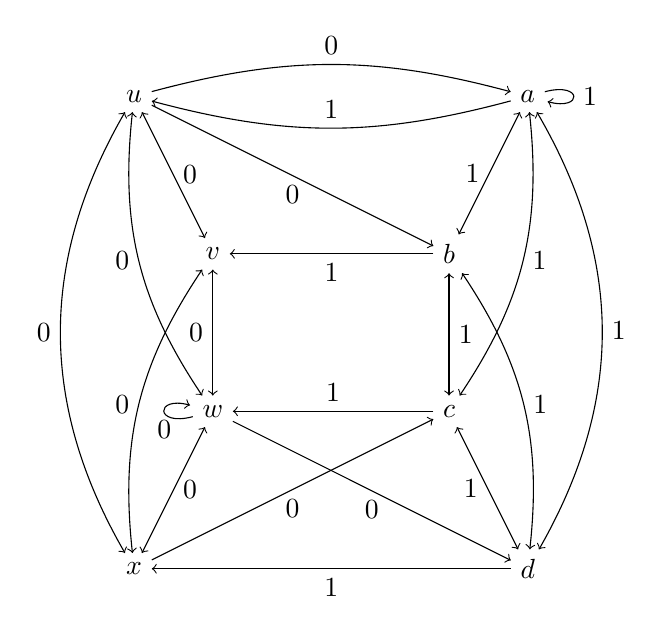
\begin{tikzpicture}
 \node (u) at (-1,6) {$u$};
 \node (v) at (0,4)  {$v$};
 \node (w) at (0,2)  {$w$};
 \node (x) at (-1,0)  {$x$};

 \node (a) at (4,6) {$a$};
 \node (b) at (3,4) {$b$};
 \node (c) at (3,2) {$c$};
 \node (d) at (4,0) {$d$};

 \draw [<->] (u) edge node [right] {$0$} (v);
 \draw [<->] (u) edge [bend right=20] node [left] {$0$} (w);
 \draw [<->] (u) edge [bend right=30] node [left] {$0$} (x);
 \draw [<->] (v) edge node [left] {$0$} (w);
 \draw [<->] (v) edge [bend right=20] node [left] {$0$} (x);
 \draw [<->] (w) edge node [right] {$0$} (x);

 \draw [<->] (a) edge node [left] {$1$} (b);
 \draw [<->] (a) edge [bend left=20] node [right] {$1$} (c);
 \draw [<->] (a) edge [bend left=30] node [right] {$1$} (d);
 \draw [<->] (b) edge node [right] {$1$} (c);
 \draw [<->] (b) edge [bend left=20] node [right] {$1$} (d);
 \draw [<->] (c) edge node [left] {$1$} (d);

 \draw [->] (w) edge [loop left] node [below] {$0$} (w);
 \draw [->] (a) edge [loop right] node [right] {$1$} (a);

 \draw [->] (u) edge [bend left=15] node [above] {$0$} (a);
 \draw [->] (u) edge node [below] {$0$} (b);
 \draw [->] (w) edge node [below] {$0$} (d);
 \draw [->] (x) edge node [below] {$0$} (c);


 \draw [->] (a) edge [bend left=15] node [above] {$1$} (u);
 \draw [->] (b) edge node [below] {$1$} (v);
 \draw [->] (c) edge node [above] {$1$} (w);
 \draw [->] (d) edge node [below] {$1$} (x);

\end{tikzpicture}
\end{center}
In this pattern there is for every word $w$ a node such that there is a
$w$-loop at the node and the node sees every other node via a $w$-path.
But it can not color any $T_n$ because in any $T_n$ the path from $01
\dots$ to $0 \dots$ is of even length and there is no even length
$01$-path from $u$ to $w$ in the pattern.

\section{Simple example}

The following seems to not allow for a homomorphism. But why?
\begin{center}
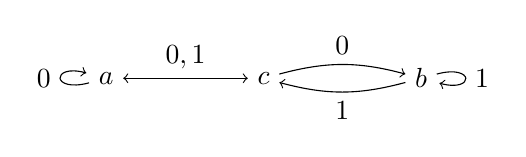
\begin{tikzpicture}
 \node (a) at (0,0) {$a$};
 \node (c) at (2,0) {$c$};
 \node (b) at (4,0)  {$b$};

 \draw [<->] (a) edge node[above] {$0,1$} (c);
 \draw [->] (a) edge [loop left] node[left] {$0$} (a);
 \draw [->] (b) edge [loop right] node[right] {$1$} (a);

 \draw [->] (c) edge [bend left=15] node[above] {$0$} (b);

 \draw [->] (b) edge [bend left=15] node[below] {$1$} (c);
\end{tikzpicture}
\end{center}



\end{document}
